\newcommand{\qsq}{\ensuremath{Q^2_{QE}}\xspace}
\renewcommand{\textfraction}{0.05}
\renewcommand{\topfraction}{0.95}
\renewcommand{\bottomfraction}{0.95}
\renewcommand{\floatpagefraction}{0.95}
\renewcommand{\dblfloatpagefraction}{0.95}
\renewcommand{\dbltopfraction}{0.95}
\setcounter{totalnumber}{5}
\setcounter{bottomnumber}{3}
\setcounter{topnumber}{3}
\setcounter{dbltopnumber}{3}

{\normalsize \appendix{Appendix: Supplementary Material}\hfill\vspace*{4ex}}

\begin{figure}[htpb]
\centering
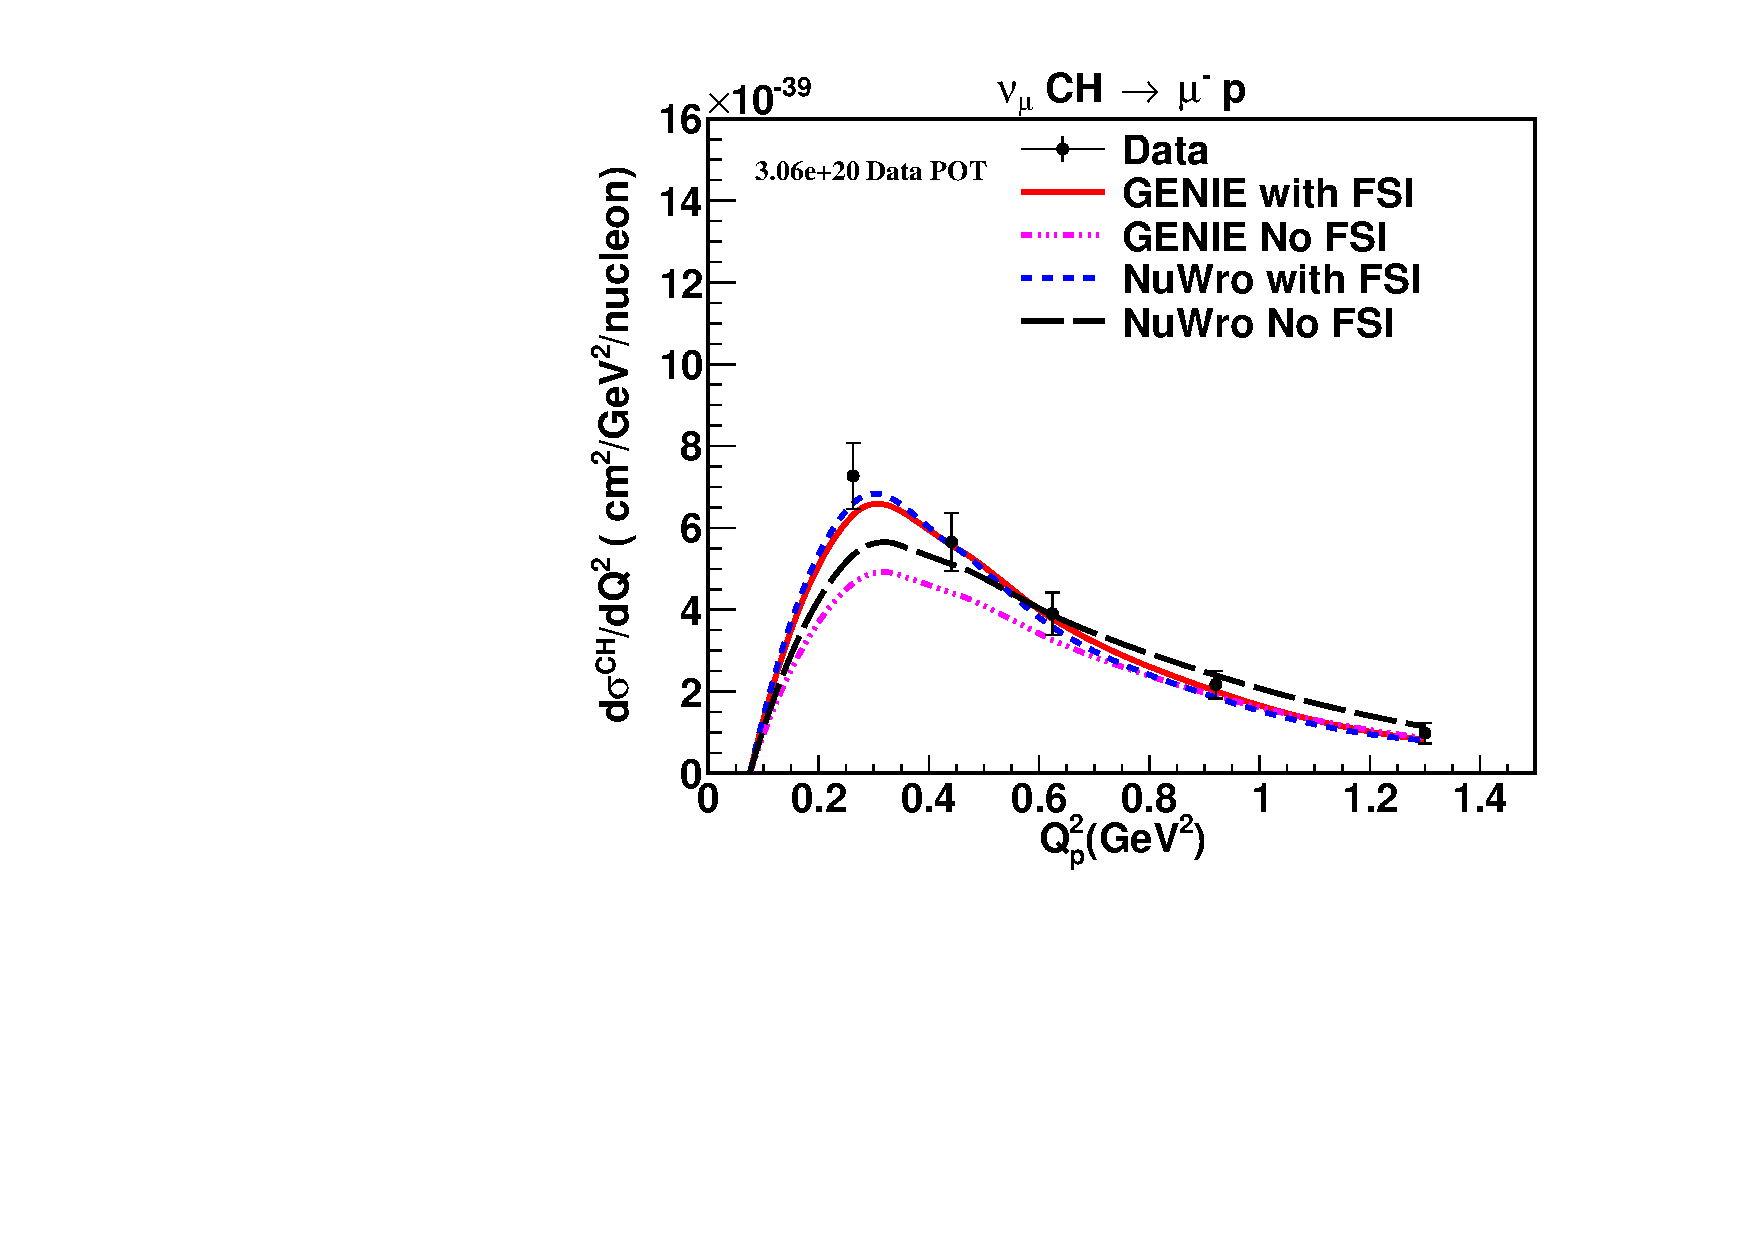
\includegraphics[trim = 0mm 4mm 10mm 2mm, clip, width=0.48\columnwidth]{DiffXsec_CH.pdf}
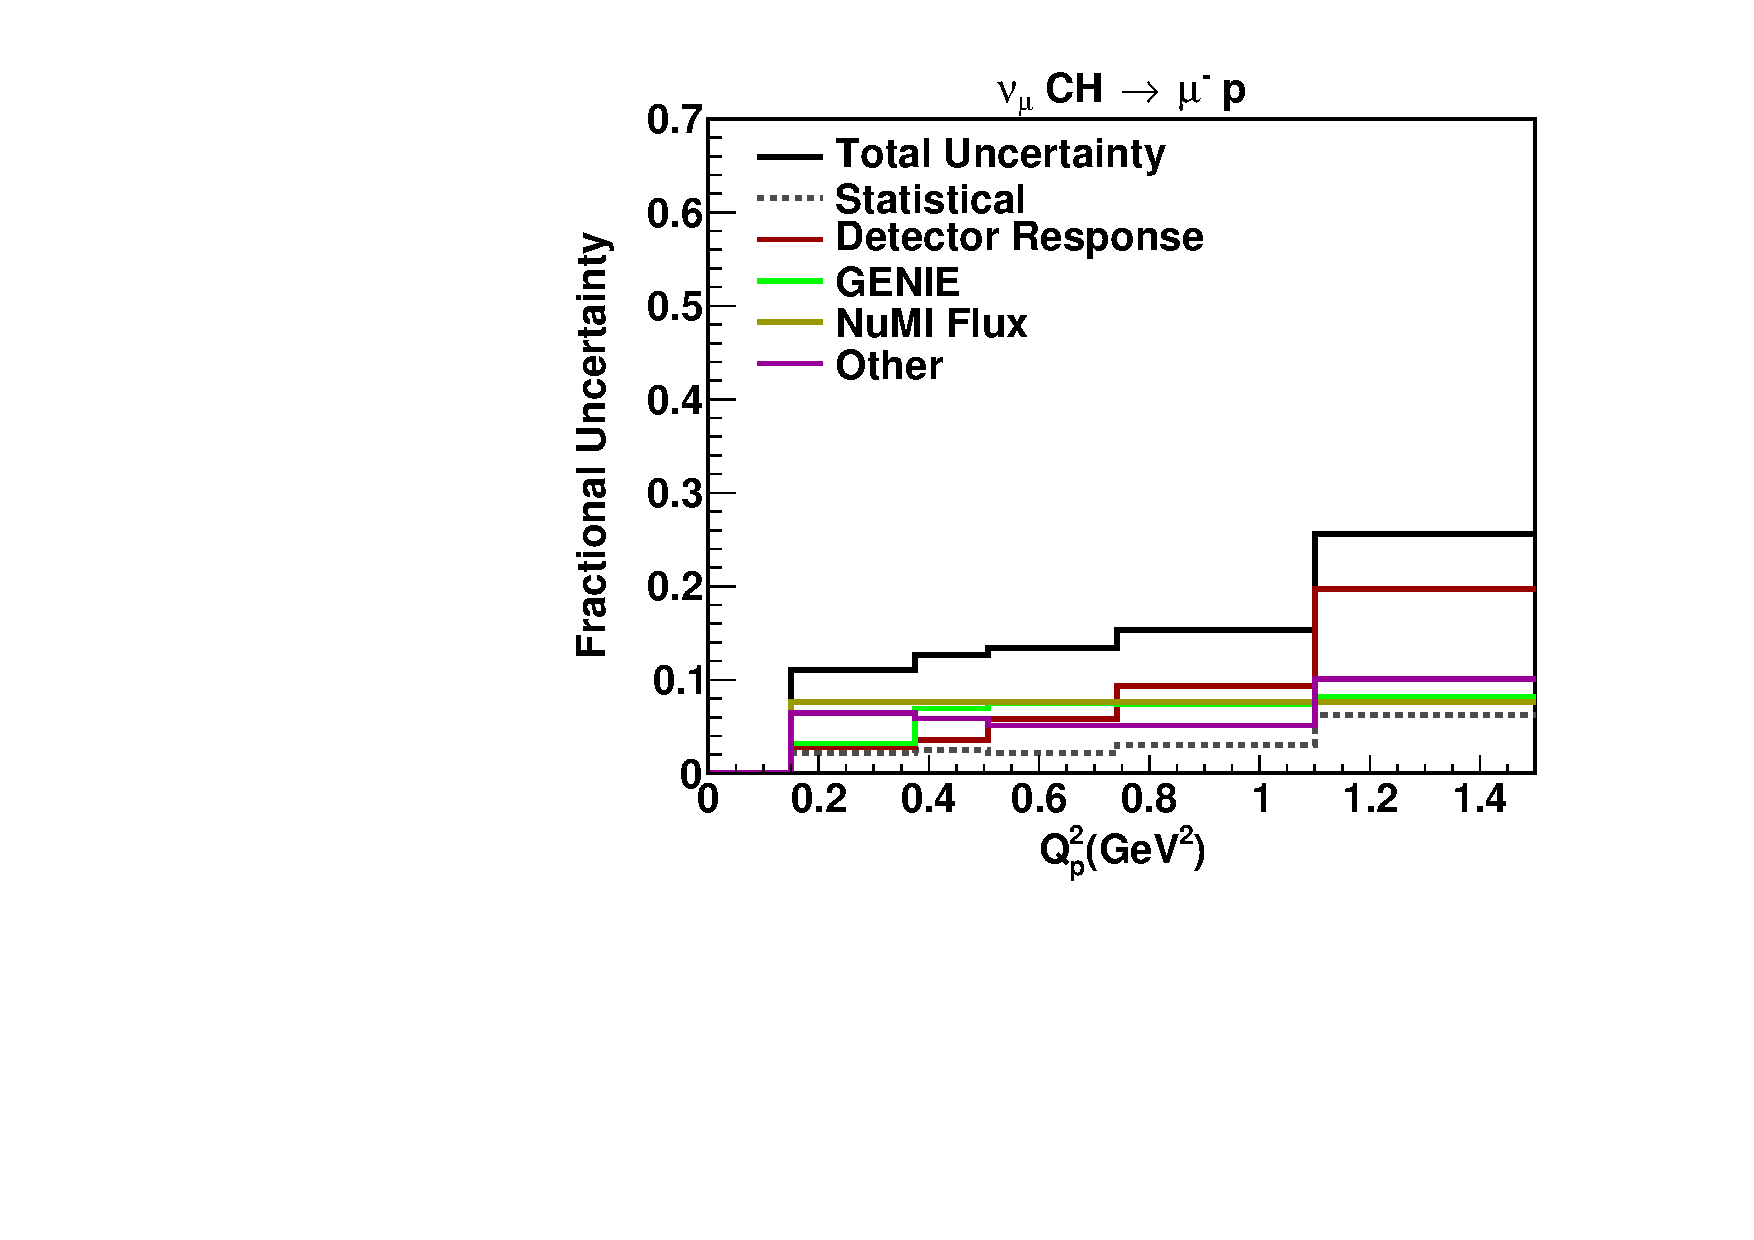
\includegraphics[trim = 0mm 4mm 10mm 2mm, width=0.48\columnwidth]{DiffXsec_CHError.pdf}
\caption{Left: Differential cross sections as a function of $Q^{2}_p$ on CH compared to predictions from \genie and \nuwro. Right: Fractional uncertainties for each bin of \QSqproton. The dashed curve shows the statistical uncertainty,  while the solid lines show individual components of the systematic uncertainty.}\label{fig:cross_section_modelCH}
\end{figure}

\begin{figure}[htpb]
\centering
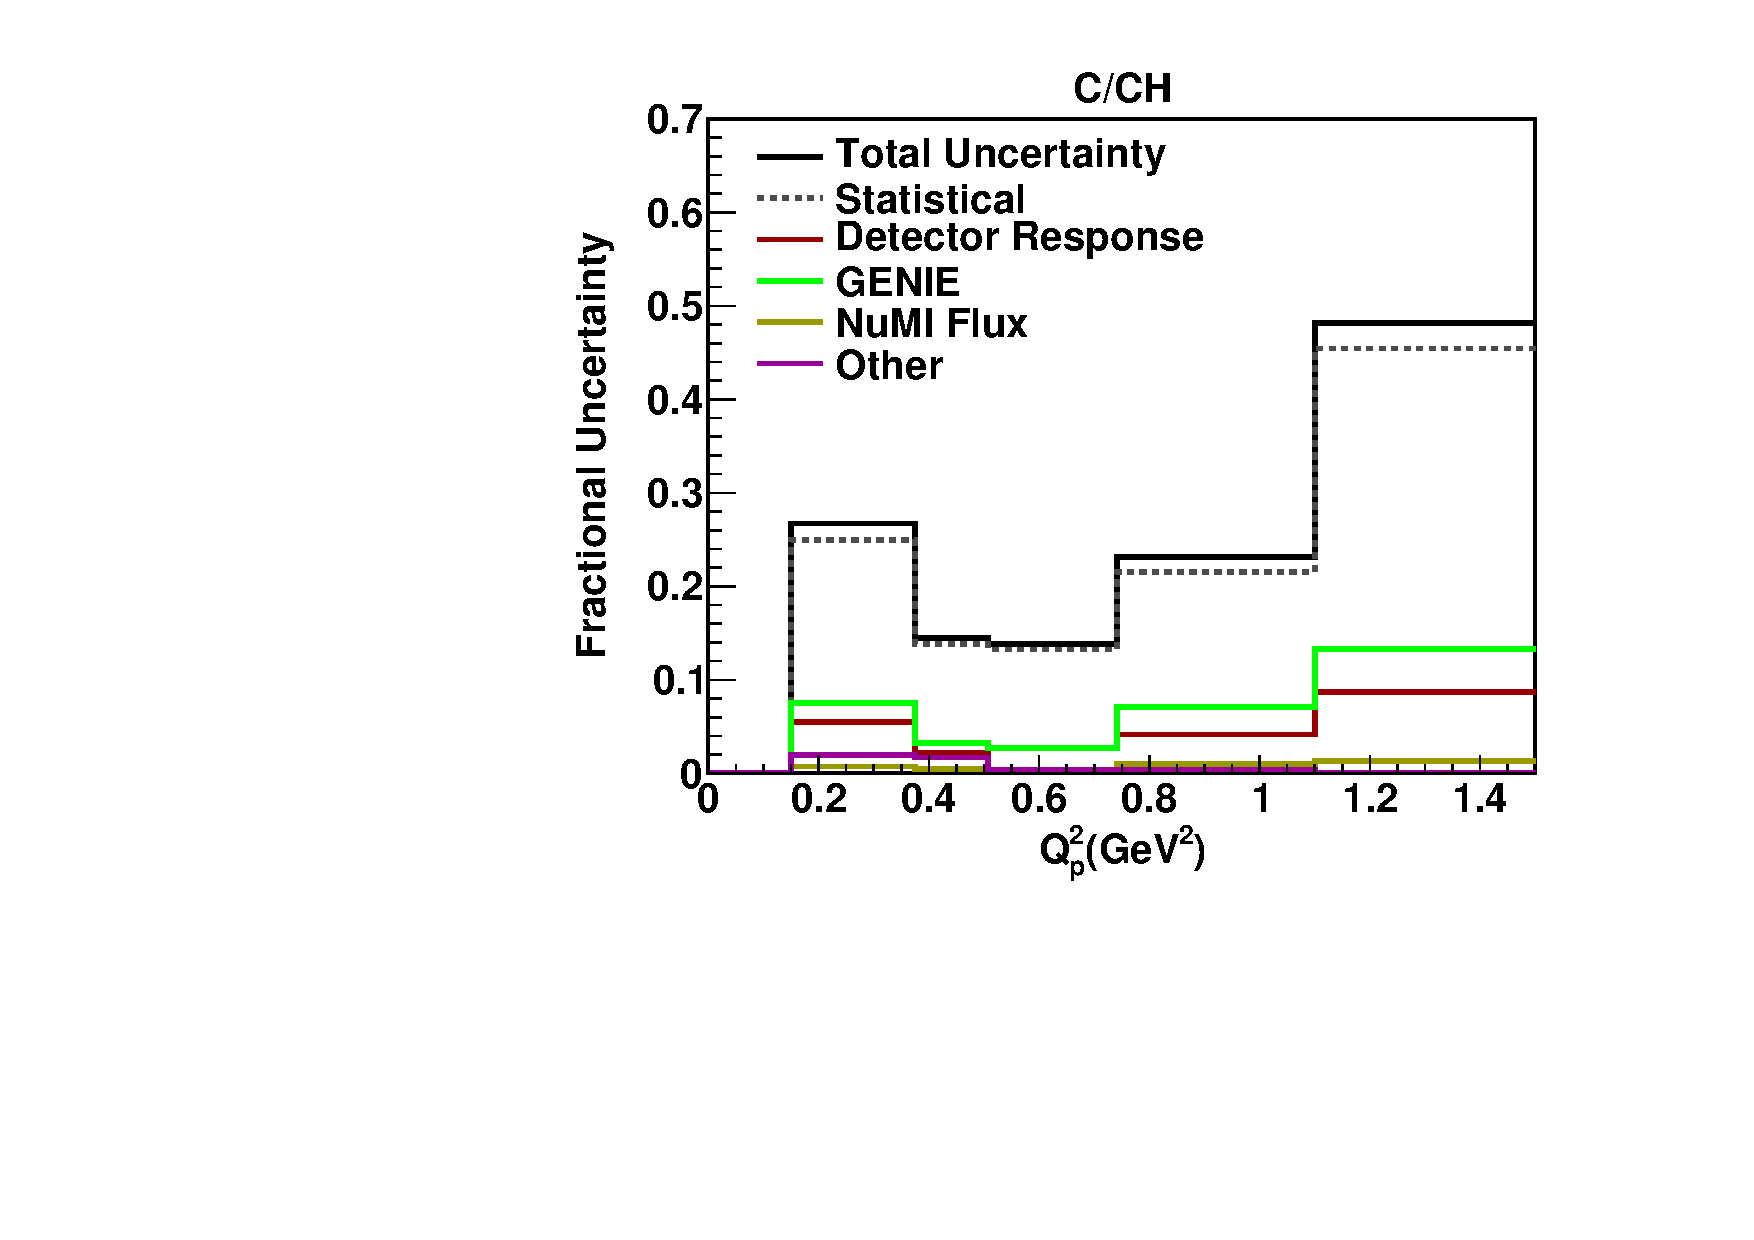
\includegraphics[trim = 2mm 8mm 15mm 8mm, width=0.48\columnwidth]{Ratio_CError.pdf}
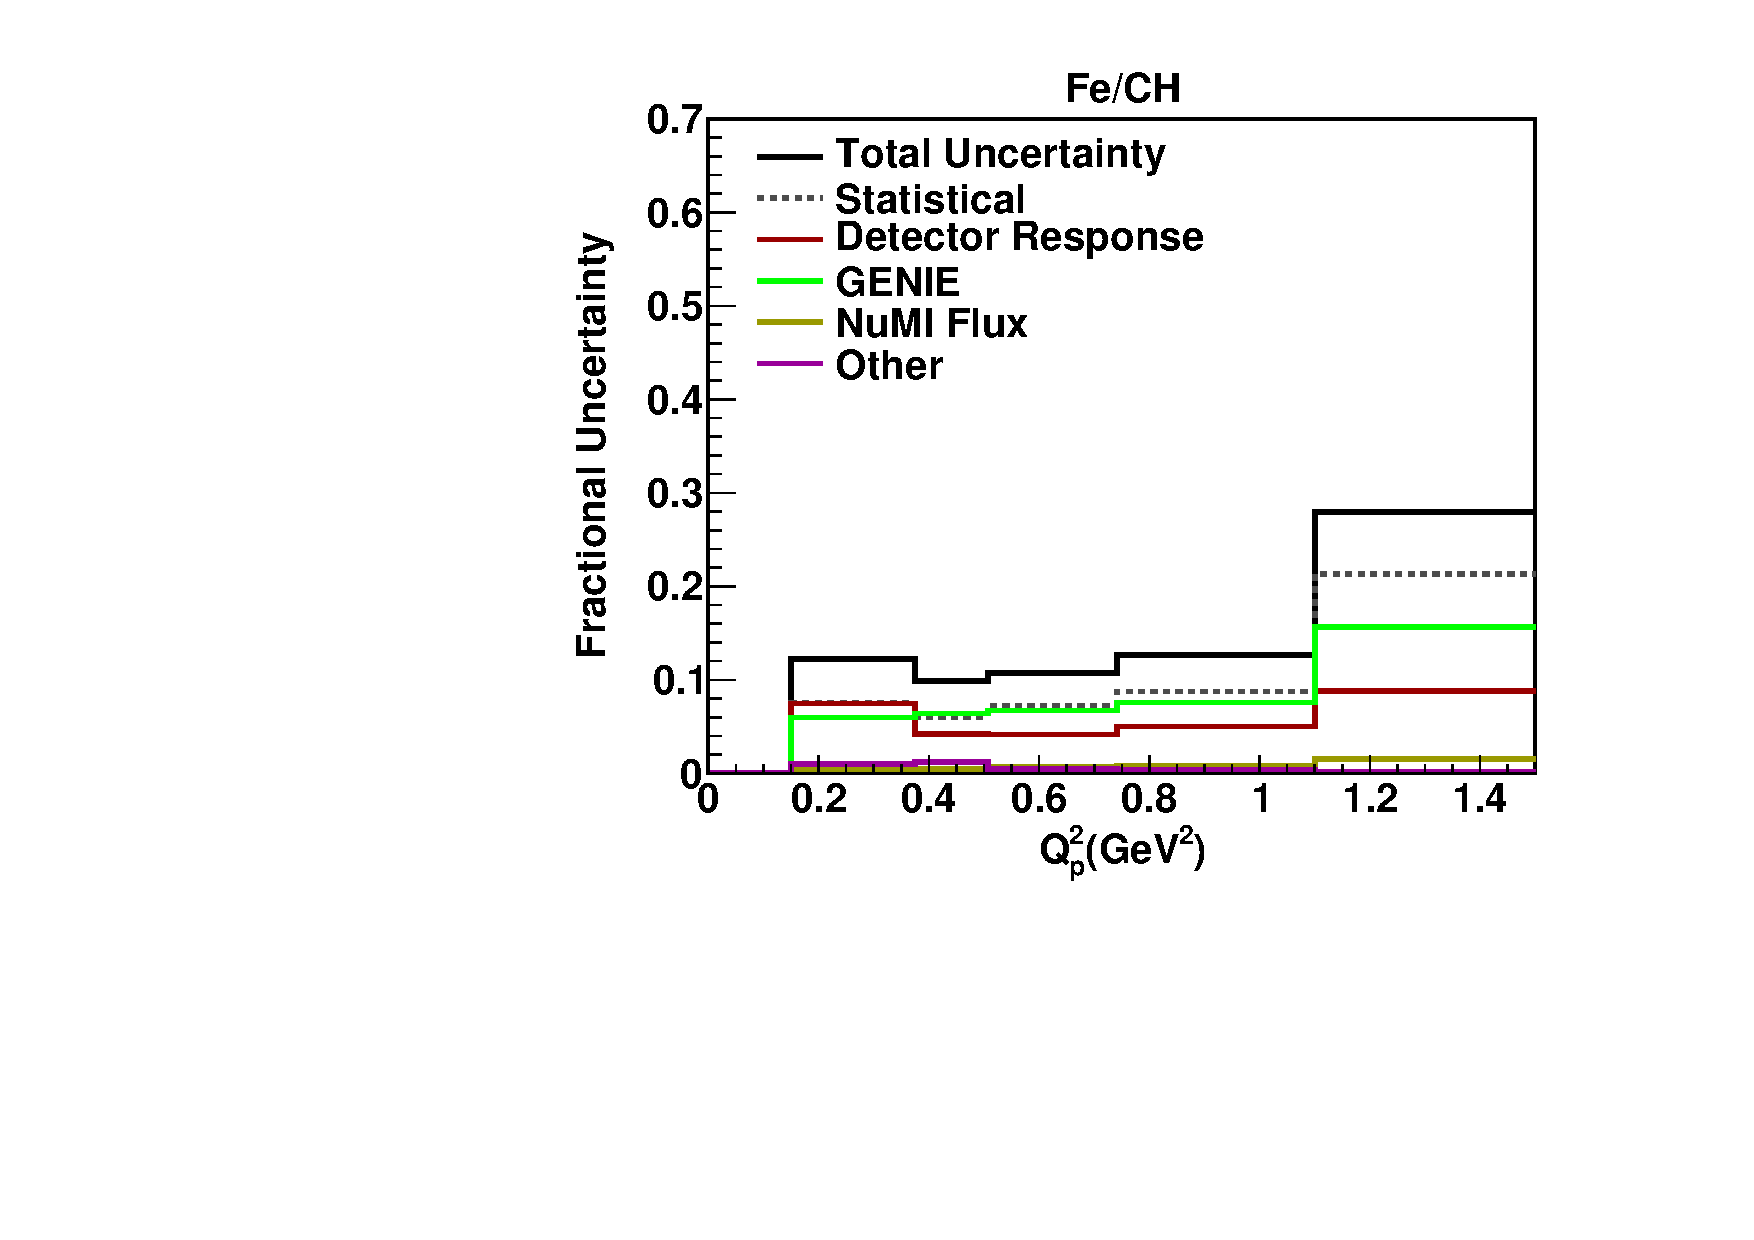
\includegraphics[trim = 2mm 8mm 15mm 8mm, width=0.48\columnwidth]{Ratio_FeError.pdf}
\caption{ Fractional uncertainties for $\frac{d\sigma}{dQ^{2}_{p}}$ as a function of $Q^2_p$ for C (left) and Fe (right); the dashed curve is from statistical and each of the contributions for the systematics.}\label{fig:cross_section_modelE}
\end{figure}

\begin{figure}[htpb]
\centering
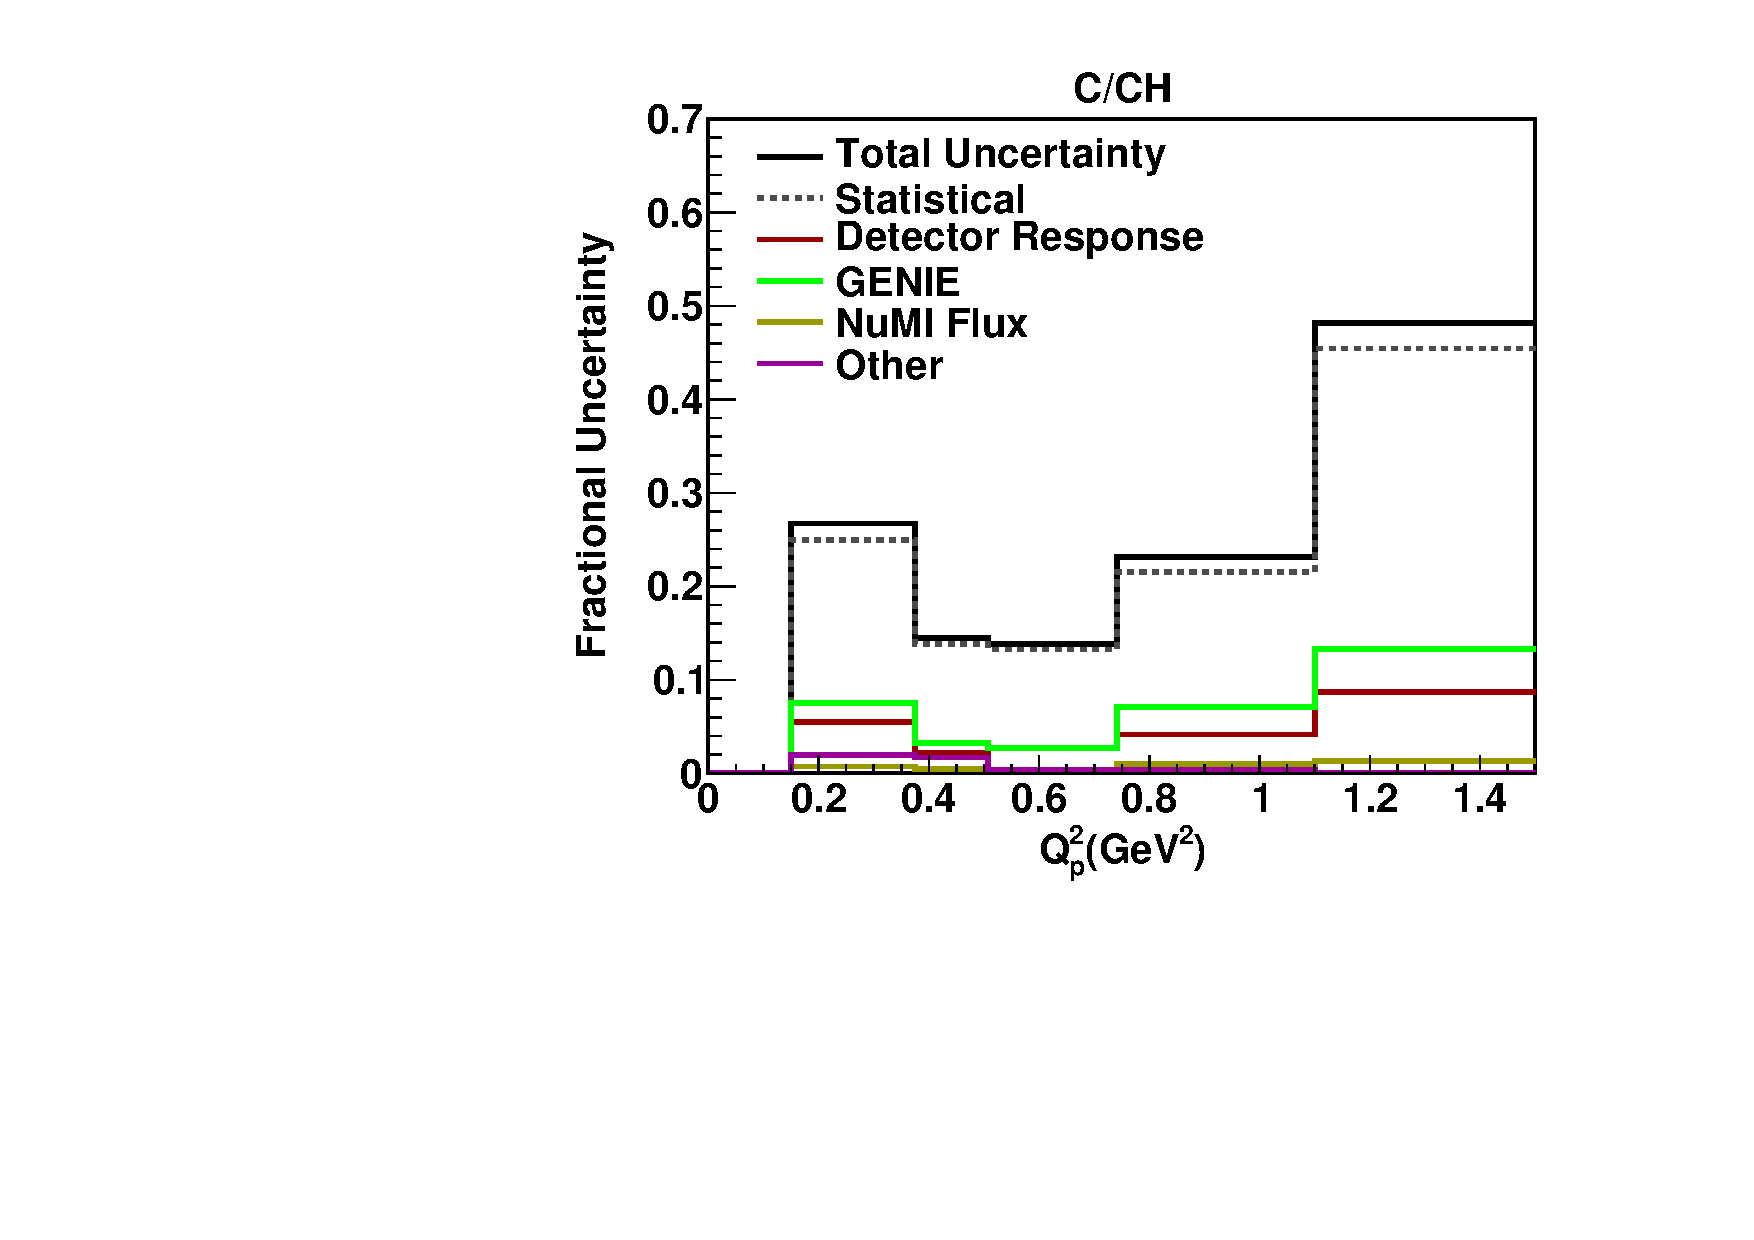
\includegraphics[trim = 2mm 8mm 15mm 8mm, width=0.48\columnwidth]{Ratio_CError.pdf}
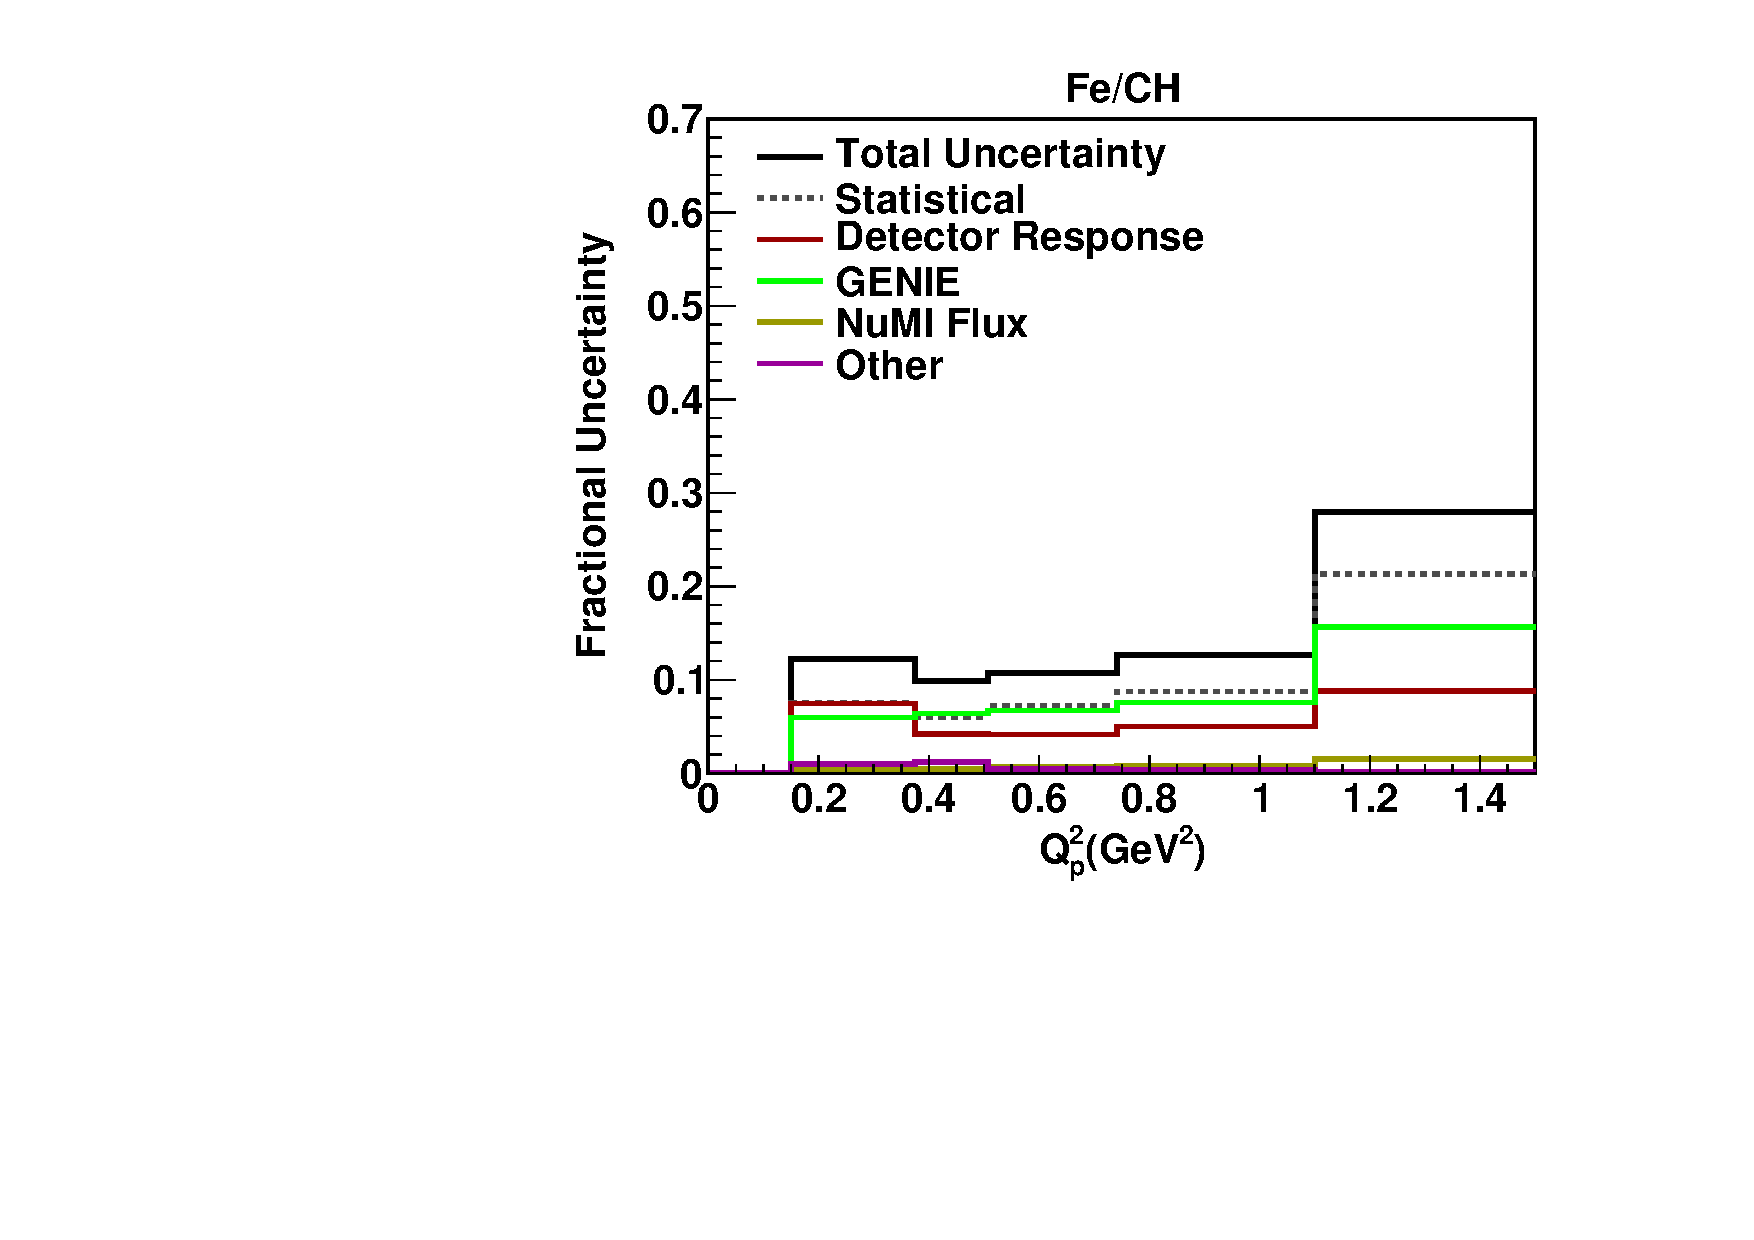
\includegraphics[trim = 2mm 8mm 15mm 8mm, width=0.48\columnwidth]{Ratio_FeError.pdf}
\caption{ Fractional uncertainties for the $\frac{d\sigma}{dQ^{2}_{p}}$ ratio as a function of $Q^2_p$ for C/CH (left) and Fe/CH (right); the dashed curve shows statistical uncertainty, the solid curves (color online) show systematic uncertainties each of the contributions for the systematics and black is the total uncertainty.}
\label{fig:ratiosE}
\end{figure}

\begin{table}[ht]
\begin{center}
    \begin{tabular}{c| c}
    \hline
\hline 
    $Q^{2}_{p}$ ($GeV^2$) & Cross section for C($10^{-38}cm^2/GeV^2$/nucleon) \\  
\hline
    0.15 - 0.375 & 0.682 $\pm$ 0.170 $\pm$ 0.101 \\  
    0.375 - 0.507 & 0.530 $\pm$ 0.072 $\pm$ 0.074\\  
    0.507 - 0.741 & 0.517 $\pm$ 0.068 $\pm$ 0.066\\  
    0.741 - 1.1 & 0.171 $\pm$ 0.037 $\pm$ 0.034\\  
    1.1 - 1.5 & 0.065 $\pm$ 0.029 $\pm$ 0.0206\\  
     \hline
\hline
    \end{tabular}
\caption{Measured \xsecproton and total uncertainties for C }

\end{center}
\end{table}

\begin{table}[ht]
\begin{center}
    \begin{tabular}{c|c}
     \hline
\hline
    $Q^{2}_{p}$ ($GeV^2$) & Cross section for Fe($10^{-38}$$cm^2$/$GeV^2$/nucleon) \\  
\hline
    0.15 - 0.375 & 1.133 $\pm$ 0.081 $\pm$ 0.157 \\  
    0.375 - 0.507 & 0.685 $\pm$ 0.038 $\pm$ 0.117\\  
    0.507 - 0.741 & 0.364 $\pm$ 0.025 $\pm$ 0.066\\  
    0.741 - 1.1 & 0.205 $\pm$ 0.017 $\pm$ 0.042\\  
    1.1 - 1.5 & 0.063 $\pm$ 0.013 $\pm$ 0.022\\  
     \hline
\hline
    \end{tabular}
\caption{Measured \xsecproton and total uncertainties for Fe }
\end{center}
\end{table}

\begin{table}[ht]
\begin{center}
    \begin{tabular}{c|c}
     \hline
\hline
    $Q^{2}_{p}$ ($GeV^2$) & Cross section for Pb ($10^{-38}$$cm^2$/$GeV^2$/nucleon) \\  
\hline
    0.15 - 0.375 & 1.057 $\pm$ 0.092 $\pm$ 0.183 \\  
    0.375 - 0.507 & 0.612 $\pm$ 0.039 $\pm$ 0.113\\  
    0.507 - 0.741 & 0.296 $\pm$ 0.025 $\pm$ 0.060\\  
    0.741 - 1.1 & 0.161 $\pm$ 0.017 $\pm$ 0.037\\  
    1.1 - 1.5 & 0.061 $\pm$ 0.012 $\pm$ 0.020\\  
     \hline
\hline
    \end{tabular}
\caption{Measured \xsecproton and total uncertainties for Pb }
\end{center}
\end{table}

\begin{table}[ht]
\begin{center}
    \begin{tabular}{c|c}
     \hline
\hline
    $Q^{2}_{p}$ ($GeV^2$) & Ratio C/CH \\  
\hline
    0.15 - 0.375 & 0.938 $\pm$ 0.234 $\pm$ 0.089 \\  
    0.375 - 0.507 & 0.94 $\pm$ 0.13 $\pm$ 0.04\\  
    0.507 - 0.741 & 1.32 $\pm$ 0.18 $\pm$ 0.0518\\  
    0.741 - 1.1 & 0.789 $\pm$ 0.170 $\pm$ 0.066\\  
    1.1 - 1.5 & 0.659 $\pm$ 0.299 $\pm$ 0.105\\  
     \hline
\hline
    \end{tabular}
\caption{Measured Ratio C/CH and total uncertainties }
\end{center}
\end{table}

\begin{table}[ht]
\begin{center}
    \begin{tabular}{c|c}
     \hline
\hline
    $Q^{2}_{p}$ ($GeV^2$) & Ratio Fe/CH \\  
\hline
    0.15 - 0.375 & 1.559 $\pm$ 0.117 $\pm$ 0.150 \\  
    0.375 - 0.507 & 1.212 $\pm$ 0.073 $\pm$ 0.0943\\  
    0.507 - 0.741 & 0.932 $\pm$ 0.067 $\pm$ 0.074\\  
    0.741 - 1.1 & 0.945 $\pm$ 0.083 $\pm$ 0.086\\  
    1.1 - 1.5 & 0.645 $\pm$ 0.138 $\pm$ 0.116\\  
     \hline
\hline
    \end{tabular}
\caption{Measured Ratio Fe/CH and total uncertainties }
\end{center}
\end{table}

\begin{table}[ht]
\begin{center}
    \begin{tabular}{c|c}
     \hline
\hline
    $Q^{2}_{p}$ ($GeV^2$) & Ratio Pb/CH  \\  
\hline
    0.15 - 0.375 & 1.454 $\pm$ 0.131 $\pm$ 0.205 \\  
    0.375 - 0.507 & 1.082 $\pm$ 0.074 $\pm$ 0.106\\  
    0.507 - 0.741 & 0.758 $\pm$ 0.066 $\pm$ 0.087\\  
    0.741 - 1.1 & 0.742 $\pm$ 0.082 $\pm$ 0.107\\  
    1.1 - 1.5 & 0.626451 $\pm$ 0.127979 $\pm$ 0.119\\  
     \hline
\hline
    \end{tabular}
\caption{Measured Ratio Pb/CH and total uncertainties }
\end{center}
\end{table}

\begin{table}[ht]
\begin{tabular}{c | c c c c c c | }
\hline
\hline
$Q^2_p$ Bins($GeV^2$)&0.15 - 0.375&0.375 - 0.507&0.507 - 0.741&0.741 - 1.1&1.1 - 1.5\\
\hline
0.15 - 0.375 & 1 & 0.78 & 0.66 & 0.57 & 0.40\\ 
0.375 - 0.507 & & 1 & 0.93 & 0.82 & 0.62 \\ 
0.507 - 0.741 & & & 1 & 0.92 & 0.75 \\ 
0.741 - 1.1 & & & &  1 & 0.86 \\ 
1.1 - 1.5 & & & & &  1  \\ 
\hline
\hline
\end{tabular}
\caption{Correlation matrix for CH}
\end{table}

\begin{table}[ht]
\begin{tabular}{c | c c c c c c | }
\hline
\hline
$Q^2_p$ Bins($GeV^2$)&0.15 - 0.375&0.375 - 0.507&0.507 - 0.741&0.741 - 1.1&1.1 - 1.5\\
\hline
0.15 - 0.375 & 1 & 0.20 & 0.21 & 0.14 & 0.09\\
0.375 - 0.507 & & 1 & 0.46 & 0.38 & 0.23 \\
0.507 - 0.741 & & & 1 & 0.41 & 0.27 \\
0.741 - 1.1 & & & &  1 & 0.36 \\
1.1 - 1.5 & & & & &  1  \\
\hline
\hline
\end{tabular}
\caption{Correlation matrix for C}
\end{table}

\begin{table}[ht]
\begin{tabular}{c | c c c c c c | }
\hline
\hline
$Q^2_p$ Bins($GeV^2$)&0.15 - 0.375&0.375 - 0.507&0.507 - 0.741&0.741 - 1.1&1.1 - 1.5\\
\hline
0.15 - 0.375 & 1 & 0.74 & 0.66 & 0.57 & 0.39\\
0.375 - 0.507 & & 1 & 0.85 & 0.75 & 0.57 \\
0.507 - 0.741 & & & 1 & 83 & 0.67 \\
0.741 - 1.1 & & & &  1 & 0.76 \\
1.1 - 1.5 & & & & &  1  \\
\hline
\hline
\end{tabular}
\caption{Correlation matrix for Fe}
\end{table}

\begin{table}[ht]
\begin{tabular}{c | c c c c c c | }
\hline
\hline
$Q^2_p$ Bins($GeV^2$)&0.15 - 0.375&0.375 - 0.507&0.507 - 0.741&0.741 - 1.1&1.1 - 1.5\\
\hline
0.15 - 0.375 & 1 & 0.78 & 0.65 & 0.46 & 0.30\\
0.375 - 0.507 & & 1 & 0.80 & 0.62 & 0.43 \\
0.507 - 0.741 & & & 1 & 0.77 & 0.60 \\
0.741 - 1.1 & & & &  1 & 0.74 \\
1.1 - 1.5 & & & & &  1  \\
\hline
\hline
\end{tabular}
\caption{Correlation matrix for Pb}
\end{table}

\begin{table}[ht]
\begin{tabular}{c | c c c c c c | }
\hline
\hline
$Q^2_p$ Bins($GeV^2$)&0.15 - 0.375&0.375 - 0.507&0.507 - 0.741&0.741 - 1.1&1.1 - 1.5\\
\hline
0.15 - 0.375 & 1 & 0.53 & 0.43 & 0.34 & 0.14\\
0.375 - 0.507 & & 1 & 0.52 & 0.44 & 0.24 \\
0.507 - 0.741 & & & 1 & 0.50 & 0.35 \\
0.741 - 1.1 & & & &  1 & 0.40 \\
1.1 - 1.5 & & & & &  1  \\
\hline
\hline
\end{tabular}
\caption{Correlation matrix for Ratio Fe/CH  }
\end{table}
\newpage
\begin{table}[ht]
\begin{tabular}{c | c c c c c c|  }
\hline
\hline
$Q^2_p$ Bins($GeV^2$)&0.15 - 0.375&0.375 - 0.507&0.507 - 0.741&0.741 - 1.1&1.1 - 1.5\\
\hline
0.15 - 0.375 & 1 & 0.61 & 0.43 & 0.22 & 0.03\\
0.375 - 0.507 & & 1 & 0.54 & 0.35 & 0.14 \\
0.507 - 0.741 & & & 1 & 0.57 & 0.38 \\
0.741 - 1.1 & & & &  1 & 0.48 \\
1.1 - 1.5 & & & & &  1  \\
\hline
\hline
\end{tabular}
\caption{Correlation matrix for Ratio Pb/CH  }
\end{table}

%\begin{table}[ht]
%\begin{tabular}{c | c c c c c c  }
%\hline
%\hline
%$Q^2_p$ Bins($GeV^2$)&0.15 - 0.375&0.375 - 0.507&0.507 - 0.741&0.741 - 1.1&1.1 - 1.5\\
%\hline
%0.15 - 0.375 & 1 & 0.61 & 0.43 & 0.22 & 0.03\\
%0.375 - 0.507 & & 1 & 0.54 & 0.35 & 0.14 \\
%0.507 - 0.741 & & & 1 & 0.57 & 0.38 \\
%0.741 - 1.1 & & & &  1 & 0.48 \\
%1.1 - 1.5 & & & & &  1  \\
%\hline
%\hline
%\end{tabular}
%\caption{Ratio Carbon/CH}
%\end{table}


